\chapter{Analysis of the Paper}
\label{C_Kapitel}
% #######################################################################
\section{one machine model}
\noindent the Figure~\ref{State transition diagram of one geometric machine} is a model of geometric machine

\begin{figure}[!h]
	\centering
	\includegraphics[]{figures/model_of_one_machine.tikz}
	\caption{State transition diagram of one geometric machine}
	\label{State transition diagram of one geometric machine}
\end{figure}

% \begin{math}x(n+1)=A_1 x(n)\end{math}
the production rate and consumption rate of an individual machine with the original state of down(0) can be calculated as 
\begin{displaymath} PR(n)=CR(n)=x_1(n)=\begin{bmatrix} 0&1 \end{bmatrix}x(n)=\begin{bmatrix} 0&1 \end{bmatrix}A_1^n
x(0) \end{displaymath}
where
\begin{displaymath} A_1 = \begin{bmatrix} 1-R&P\\R&1-P \end{bmatrix} \end{displaymath}

the Figure~\ref{Transients of an individual geomatric machine when it is initially down} is the contrast of simulation and calculation of one geometric machine with initial state of down with the parameters of breakdown
probability $P = 0.05$ and repair probability $R = 0.2$.

\begin{figure*}[!h]
	\centering
	\subfigure[Result of simulation]{
		\includegraphics[width=6.5cm]{figures/individual_s_0.tikz}
		\label{individual simulation down}}
	\subfigure[Result of calculation]{
		\includegraphics[width=6.5cm]{figures/individual_c_0.tikz}	
	 	\label{individual calculation down}}
	\caption{Transients of an individual geomatric machine when it is initially down}
	\label{Transients of an individual geomatric machine when it is initially down}
\end{figure*}

the Figure~\ref{Transients of an individual geomatric machine when it is initially up} is the contrast of simulation and calculation of one geometric machine with initial state of up and the paramter is same with the fore figure

\begin{figure*}[!h]
	\centering
	\subfigure[Result of simulation]{
		\includegraphics[width=6.5cm]{figures/individual_s_1.tikz}
		\label{individual simulation up}}
	\subfigure[Result of calculation]{
		\includegraphics[width=6.5cm]{figures/individual_c_1.tikz}	
	 	\label{individual calculation up}}
	\caption{Transients of an individual geomatric machine when it is initially up}
	\label{Transients of an individual geomatric machine when it is initially up}
\end{figure*}

\section{two machine model}
\noindent the Figure~\ref{State transition diagram of two geometric machine with buffer} is the mathmatic model of two machine geometric serial line 
\begin{figure}[!h]
	\centering
	\includegraphics[]{figures/model_of_two_machine_with_buffer.tikz}
	\caption{State transition diagram of two geometric machine with buffer}
	\label{State transition diagram of two geometric machine with buffer}
\end{figure}

the Figure~\ref{Transients of a two-machine geometric line} is the the result of simulation of two machine with buffer with the paramters of $P_1 = 0.03, R_1 = 0.18, P_2 = 0.06, R_2 = 0.21,$ Buffer $ N = 10$.

\begin{figure*}[!h]
	\centering
	\subfigure[]{
		\includegraphics[width=0.45\linewidth,height=0.35\linewidth]{figures/two_machine_pr_and_cr.tikz}
		\label{two machine pr and cr}}
	\subfigure[]{
		\includegraphics[width=0.45\linewidth,height=0.35\linewidth]{figures/two_machine_wip.tikz}	
		 \label{two machine wip}}
	\subfigure[]{
		\includegraphics[width=0.45\linewidth,height=0.35\linewidth]{figures/two_machine_bl_and_st.tikz}	
		\label{two machine bl and st}}
	\caption{Transients of a two-machine geometric line. (a) $PR(n)\ and\ CR(n)$;(b) $WIP(n)$; (c) $ST_2(n)\ and\ BL_2(n)$}
	\label{Transients of a two-machine geometric line}
\end{figure*}
~\\
a significant difference can be found between the Figure~\ref{two machine bl and st} and the original Figure~\ref{st_bl_origin}


\begin{figure*}[!h]
	\centering
	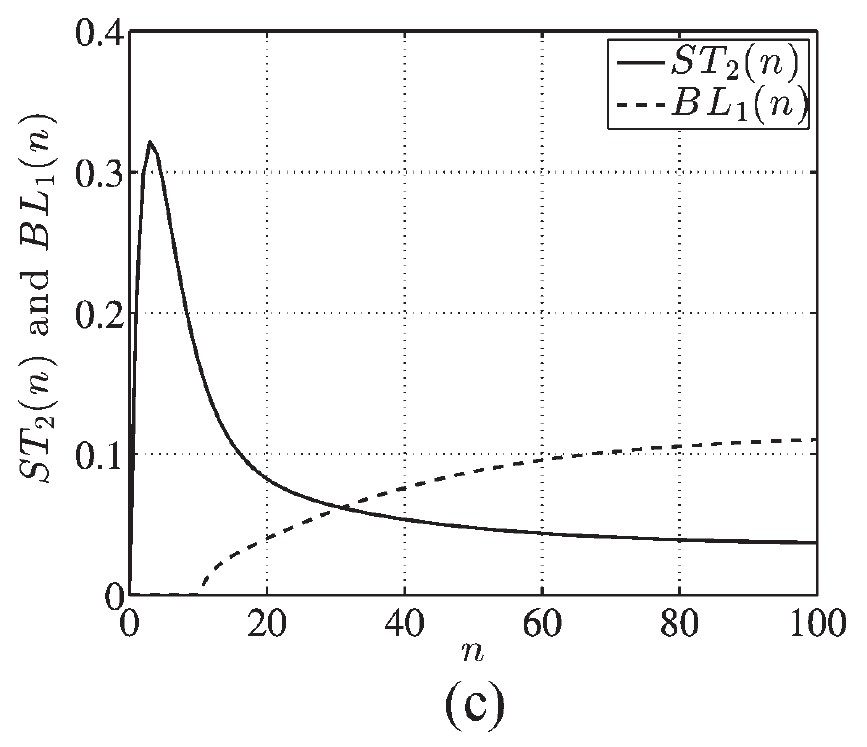
\includegraphics[width=0.45\linewidth]{figures/st-bl-origin.jpg}
	\caption{Transients of a two-machine geometric line $ST_2(n) \ and\ BL_2(n)$}
	\label{st_bl_origin}
\end{figure*}

~\\
Parameters of aggregated machines in a two-machine geometric
serial line.

\begin{figure*}[!h]
	\centering
	\includegraphics[width=0.45\linewidth]{figures/two_machine_aggregated.tikz}
	\caption{Parameters of aggregated machines in a two-machine geometric serial line.}
	\label{two machines aggregated}
\end{figure*}

\section{multi machine model}
\noindent the following is the part about multi geometric machines with four machine and the parameters are 
$P_i = 0.05, R_i = 0.2, i = 1,...,4; N_i = 5, i = 1,...,3.$

\begin{figure*}[!h]
	\centering
	\subfigure[]{
		\includegraphics[width=0.45\linewidth,height=0.35\linewidth]{figures/four_machine_pr_and_cr.tikz}
		\label{four machine pr and cr}}
	\subfigure[]{
		\includegraphics[width=0.45\linewidth,height=0.35\linewidth]{figures/four_machine_wip.tikz}	
		 \label{four machine wip}}
	\subfigure[]{
		\includegraphics[width=0.45\linewidth,height=0.35\linewidth]{figures/four_machine_st.tikz}	
		\label{four machine st}}
	\subfigure[]{
		\includegraphics[width=0.45\linewidth,height=0.35\linewidth]{figures/four_machine_bl.tikz}	
		\label{four machine bl}}
	\caption{Transients of a four-machine geometric line. (a) $PR(n) \ and\ CR(n)$;(b) $WIP(n)$; (c) $ST_i(n)$;(d) $BL_i(n)$.}
	\label{Transients of a four-machine geometric line}
\end{figure*}

meanwhile, the original figures show the result of the writer